\documentclass[11pt]{article}
\usepackage[utf8]{inputenc}
\usepackage[T1]{fontenc}
\usepackage{graphicx}
\usepackage{grffile}
\usepackage{longtable}
\usepackage{wrapfig}
\usepackage{rotating}
\usepackage[normalem]{ulem}
\usepackage{amsmath}
\usepackage{textcomp}
\usepackage{amssymb}
\usepackage{capt-of}
\usepackage{hyperref}
\usepackage{minted}
\usepackage[section]{placeins}
\author{Student: Brian Cheung bc32427 \\ Professor: Mohit Tiwari \\ TA: Antonio Espinoza \\ Department of Electrical \& Computer Engineering \\ The University of Texas at Austin}
\date{\today}
\title{EE379K Enterprise Network Security Lab 1 Report}
\hypersetup{
 pdfauthor={Student: Brian Cheung bc32427 \\ Professor: Mohit Tiwari \\ TA: Antonio Espinoza \\ Department of Electrical \& Computer Engineering \\ The University of Texas at Austin},
 pdftitle={EE379K Enterprise Network Security Lab 1 Report},
 pdfkeywords={},
 pdfsubject={},
 pdfcreator={},
 pdflang={English}}
\begin{document}

\maketitle
\section*{Part 1 - Server and Client Networking}
\label{sec:part-1}
The task was to implement an echo server and client in C given a Python implementation that modeled the desired behavior of the server and client.
The Python implementation was also used to test the compatibility of the C program by interchanging the server and client with a Python server and C client and vice versa.
The next task was to perform a Denial of Service (DOS) attack on the C server.
\subsection*{Step 1 - Echo Server}
\subsubsection*{Build server and client}
In a terminal window, start at root directory of project and run the following commands:
\begin{minted}{bash}
  $ cd Part\ 1
  $ make
\end{minted}
\subsubsection*{Run server and client}
Run the following commands to start the server:
\begin{minted}{bash}
  $ cd Part\ 1
  $ ./server
\end{minted}
Open a new terminal window and run the following commands to start the client:
\begin{minted}{bash}
  $ cd Part\ 1
  $ ./client
\end{minted}
\subsection*{Step 2 - DOS Attack}
The DOS attack was performed using a program called \textbf{\emph{hping3}}.
The attacker flooded the server with SYN packets while using a spoofed IP address to hide the source IP address.
The server attempted to send the SYN and ACK packets back to the to the random spoofed IP address, but because they are spoofed,
no real client actually responded to the server
which prevented the three-way handshake from being completed.
Furthermore, this prevents the server from processing other clients' requests because it is too busy trying to complete the attacker's requests,
so clients that want to connect to the server are left waiting to complete a three-way handshake until their requests time out.

The following command was used to perform the DOS attack:
\begin{minted}{bash}
  $ sudo hping3 -S -w 64 -p 12000 --flood --rand-source 127.0.0.2
\end{minted}
\textbf{\emph{hping3}} command flags and options:

\textbf{-S}: flood with SYN packets

\textbf{-p}: 12000: port 12000

\textbf{--flood}: send packets as fast as possible

\textbf{--rand-source}: generates a spoofed IP address to hide the source IP

\textbf{127.0.0.2}: IP address of server
\newline

The recorded pcap of the attack displays the flood of SYN packets sent to the server (shown in Figure \ref{fig:client-attempt-flood})
along with the server attempting send SYN and ACK packets back to the client.
However, the server sends the packets to the spoofed IP of the attacker instead,
which prevents the three-way handshake between the server and client from being completed.
As a result, the client's request times out (shown in Figure \ref{fig:filtered-dos}).

\begin{figure}[h]
\centering
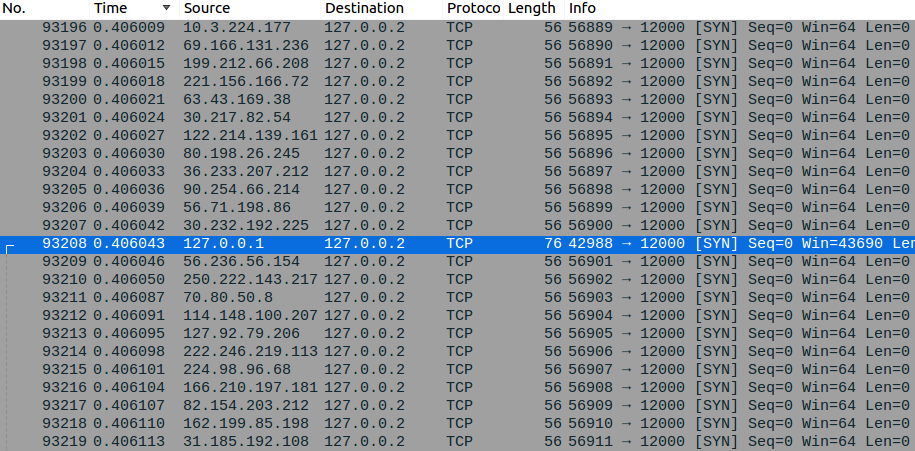
\includegraphics[width=.9\linewidth]{./client-attempt-flood.png}
\caption{\label{fig:client-attempt-flood}
Client with IP address of 127.0.0.1 attempts to connect to the server during a DOS attack.}
\end{figure}

\begin{figure}[h]
\centering
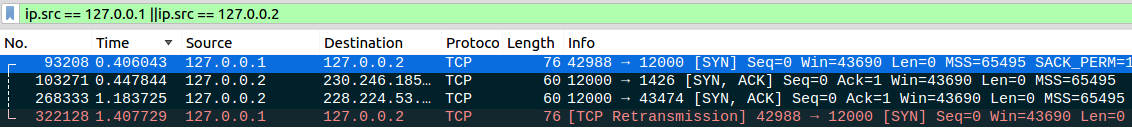
\includegraphics[width=.9\linewidth]{./filtered-dos.png}
\caption{\label{fig:filtered-dos}
The server sends SYN and ACK packets to the spoofed IP of the attacker and the client's request times out.}
\end{figure}

\section*{Part 2 - Scan the Internet}
\label{sec:part-2}
The objective of this part was to scan the internet with zmap and group IP addresses in the same network.
\subsection*{ZMAP scan}
The first step required a 2-4 hour zmap scan in order to obtain a list of IP addresses that responded when probed.

The following command was used to perform the zmap scan for three hours:
\begin{minted}{bash}
  $ sudo zmap \
      --bandwidth=1M \
      --target-port=80 \
      --blacklist-file=blacklist.txt \
      --output-file=zmap_scan.csv \
      -t 10800
\end{minted}
ZMAP scan results:

\textbf{Total number of machines probed}: 16063066

\textbf{Number of machines that responded}: 11448

\textbf{Hitrate}: 0.071\%
\newline

The next task was to group together all the IP addresses that belong in the same network.
Each network has a range of IP addresses that are defined by the network's Classless Inter-Domain Routing (CIDR).
The whois command was used to obtain the CIDR that each IP address belonged in, however,
some whois outputs have different fields that define the CIDR (CIDR, inetnum, and IPv4 Address), which complicated the parsing process.
With 11,448 IP addresses, this task was automated with a Python script (Part 2/scan/scan\_networks.py) that kept track of the IP addresses that successfully or unsuccessfully returned the desired network information.
The Python script ran a Bash script (Part 2/scan/whois\_scan.sh) in a 'subprocess' in order to obtain the desired network information from each IP address.
The output of these scripts is contained in the whois\_output.txt file (Part 2/scan/results/whois\_output.txt).

After scanning and collecting all the required data, the next step was to group and count the IP addresses in each network.
This task was also automated using a python script (Part 2/analyze/analyze\_networks.py). 
The outputs of this script is contained in the directory: Part 2/analyze/results.

\textbf{networks.json}: 16063066

\textbf{network\_ip.json}: 11448

\textbf{multiple\_cidrs.json}: 0.071\%

\textbf{subnets.json}: 0.071\%

\section*{Part 3}
\label{sec:part-3}
part 3 paragraph

\section*{Conclusion}
\label{sec:conclusion}
Please provide feedback so we can improve the labs for the course. How many
hours did the lab take you? Was this lab boring? Did you learn anything? Is
there anything you would change? Feel free to put anything here, but leaving it
blank will result in the loss of points.

\nocite{*}
\bibliography{bibliography}
\bibliographystyle{ieeetr}
\end{document}
